\chapter{Conclusioni}
Concluderemo ora il lavoro con l'analisi dei risultati ottenuti e con la discussione dei possibili sviluppi futuri.
\section{Test}
\subsection{Test con il modello prova.obj e teapot.obj}
Analizziamo i risultati ottenuti con i modelli prova.obj e teapot.obj. Le immagini \ref{img:final_tex_test_1}, \ref{img:final_tex_test_2}  e \ref{img:final_tex_teapot} rispecchiano il risultato ottenuto nella fase di packing delle superfici del modello prova.obj e del modello teapot.obj. 

\begin{figure}[!h]
\centering %
\subfigure[texture sfera di prova.obj]{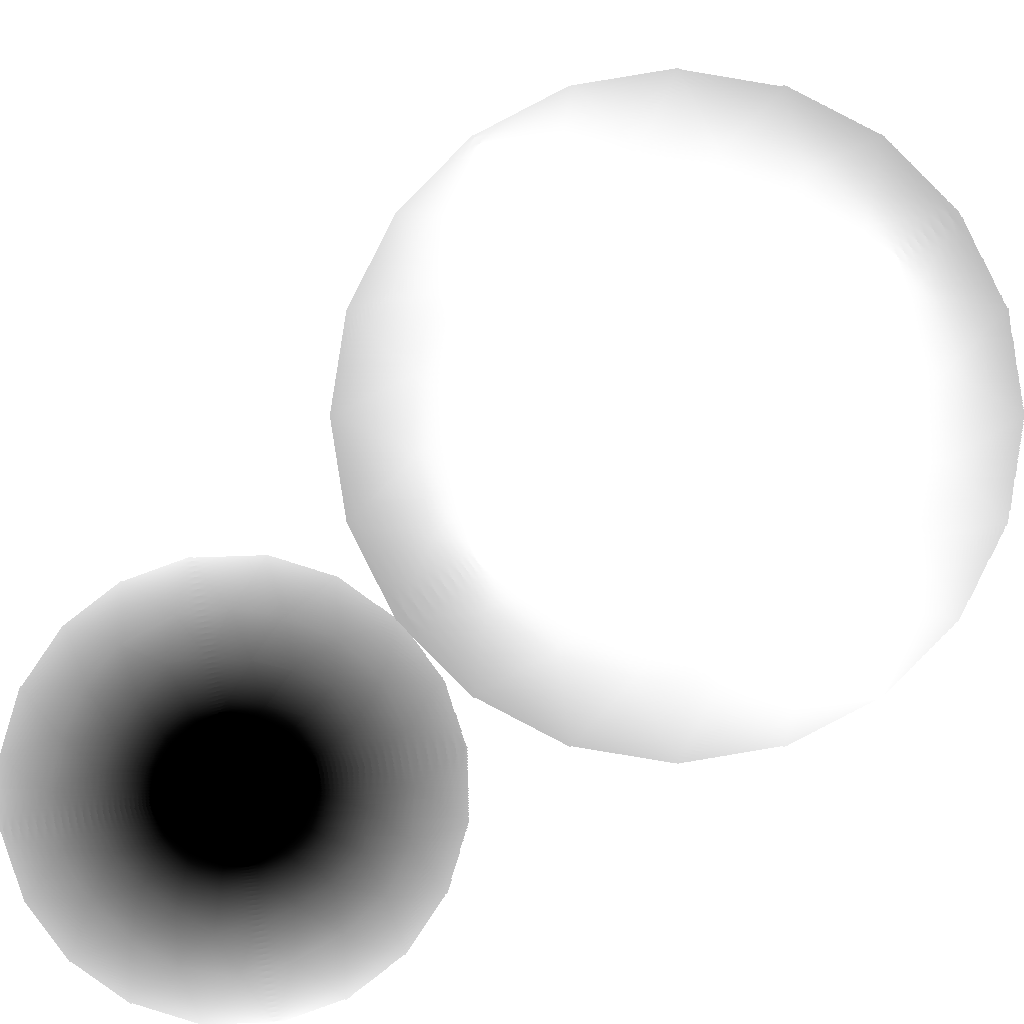
\includegraphics[scale=0.10]{images/final/test/texture_sphere.png} \label{img:final_tex_test_1}}\qquad 
\subfigure[texture piano di prova.obj]{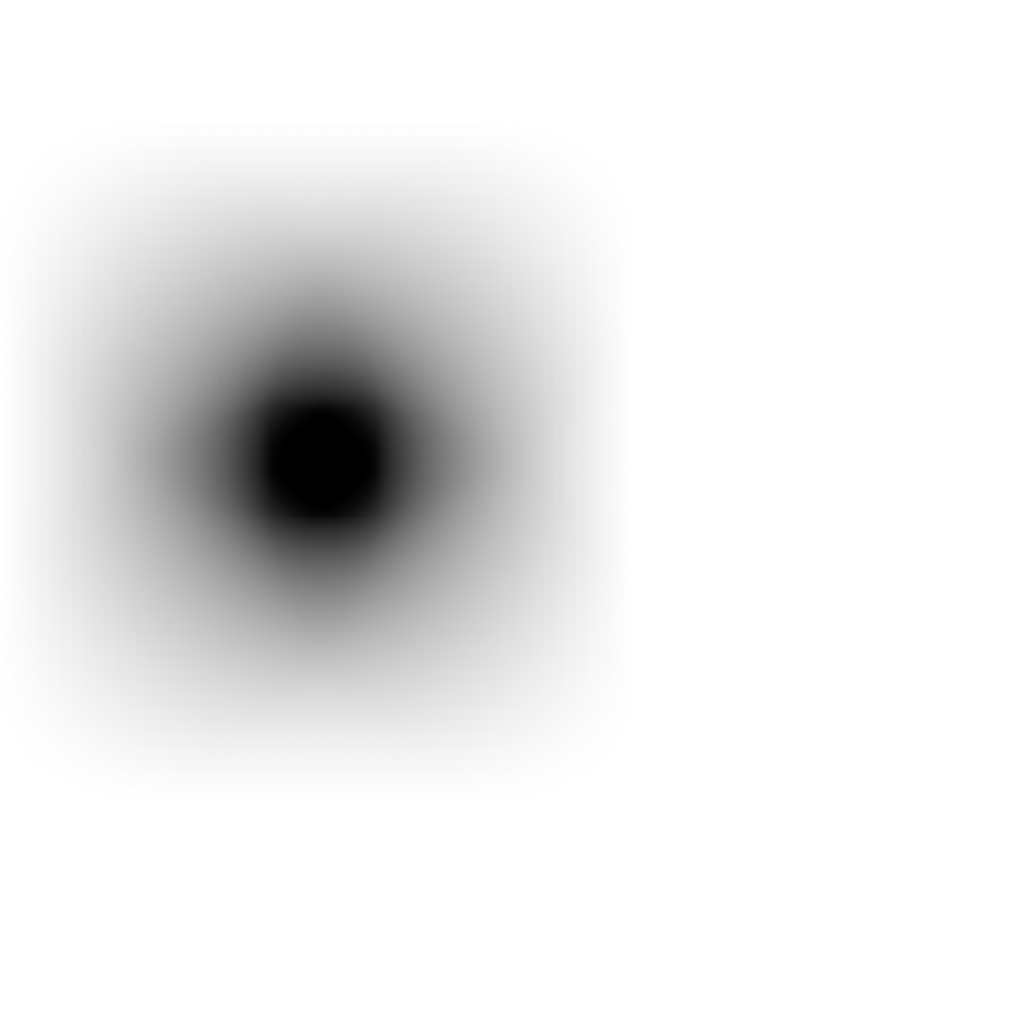
\includegraphics[scale=0.10]{images/final/test/texture_plan.png} \label{img:final_tex_test_2}} \qquad
\subfigure[texture di teapot.obj]{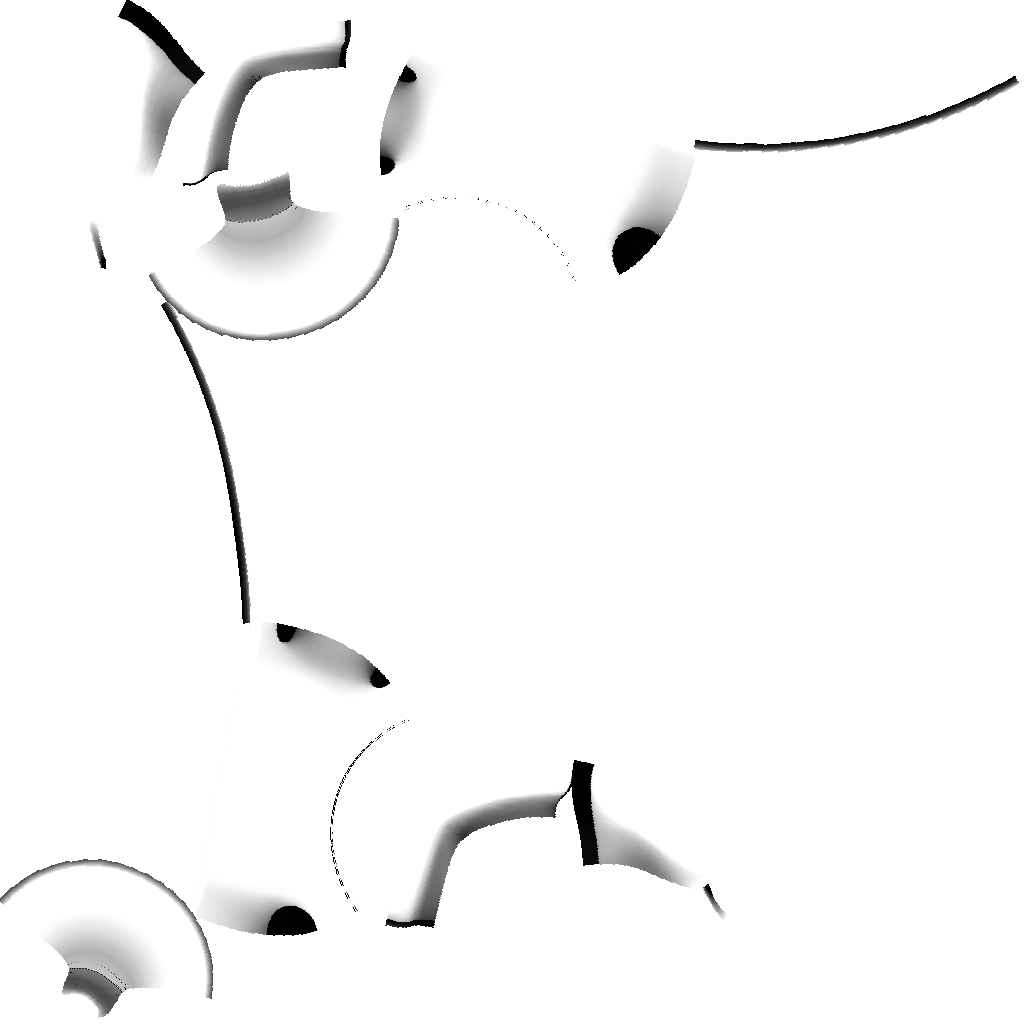
\includegraphics[scale=0.10]{images/final/teapot/texture.png} \label{img:final_tex_teapot}}
\caption{AO texture del modello prova.obj e teapot.obj}
\end{figure}


Il risultato dell'disposizione ottenuta per il modello prova.obj sembra minimizzare lo spazio non utilizzato nel quadrato, possiamo quindi supporre che per questo modello il programma generi una soluzione molto vicina all'ottimo. Mentre la disposizione ottenuta per il modello teapot.obj potrebbe essere sicuramente migliorata.

La \figurename{ \ref{img:final_tex_test_1}, \ref{img:final_tex_test_2}}  e la \figurename{ \ref{img:final_tex_teapot}} rappresentano gli output della fase di calcolo dell'AO texture per i due modelli. Il risultato ovviamente rispecchia sempre ci� che si � ottenuto nella fase di packing. Pi� avanti tratteremo in dettaglio i tempi necessari al calcolo della texture, decisamente influenti in termini di prestazioni.

Il risultato finale per i due modelli si pu� vedere nella \figurename{ \ref{img:final_out}}. In entrambi i casi i problemi riscontrati con la prima versione del programma non si sono presentati se non in minima parte, possiamo quindi concludere che le speculazioni sulle motivazioni alla base delle problematiche riscontrate erano corrette.

\begin{figure}[!h]
\centering %
\subfigure[modello prova.obj]{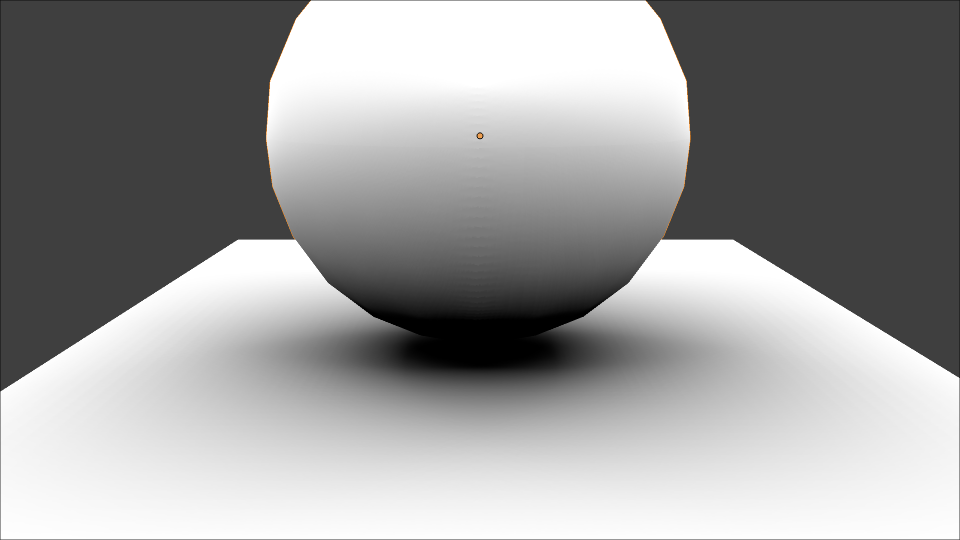
\includegraphics[scale=0.20]{images/final/test/test.png}}\qquad
\subfigure[modello teapot.obj]{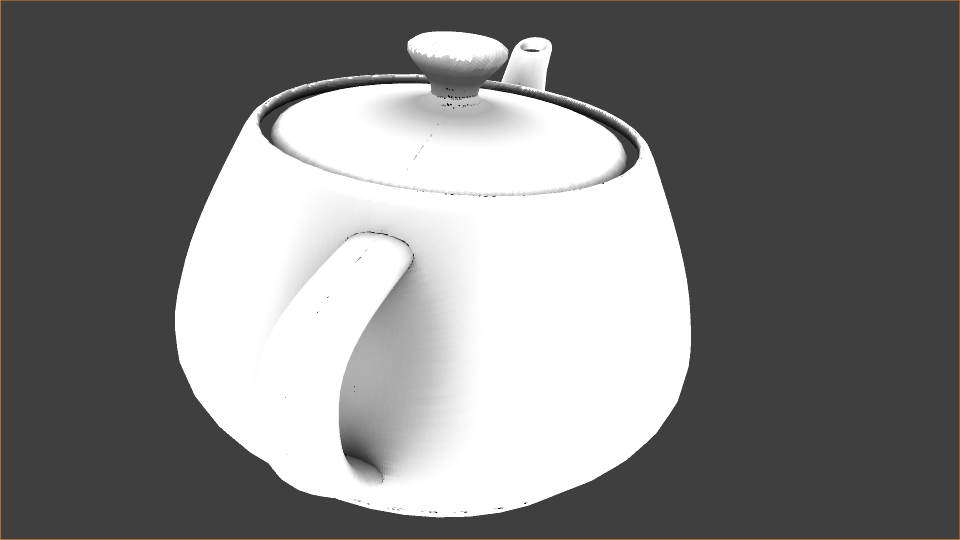
\includegraphics[scale=0.20]{images/final/teapot/teapot.png}}
\label{img:final_out}
\caption{output finale}
\end{figure}

\subsection{Test con il modello monkey.obj}
Il test con il modello monkey.obj non ha ottenuto risultati soddisfacenti. La fase in unwrapping non ha ottenuto una parametrizzazione valida per la mesh. Infatti, una sotto-superficie della mesh ha prodotto una mappatura non localmente biunivoca e quindi non valida. Nell'immagine 

\subsection{Tempi di esecuzione}
Le tempistiche di esecuzione sono certamente un punto importante per valutare se il programma � realmente in grado di risolvere il problema. L'obiettivo era quello di valutare il programma nel suo complesso , in particolare nella fase di calcolo della texture e in quella di unwrapping. 

Per valutare le prestazione dell'algoritmo per il calcolo dell'AO texture abbiamo effettuato una serie di test su un unico modello prova.obj. Le prove sono state eseguite impostando diverse risoluzioni per la texture in output, nella \tablename{ \ref{tbl:final_time_tex}} � presente il riepilogo dei dati.

\begin{table}
\centering
\renewcommand\arraystretch{1.3} % aumenta spaziatura tra le righe
\begin{tabular}{p{0.13\textwidth} | p{0.18\textwidth} | p{0.18\textwidth} | p{0.18\textwidth} | p{0.18\textwidth}}
	\textbf{Fase} & \textbf{lato 256px} & \textbf{lato 512px} & \textbf{lato 1024px} & \textbf{lato 2048px} \\
	\hline
	Unwrapping  & 6.5990 s & 6.5830 s & 6.5670 s & 6.5540 s \\

	Packing & 0.8740 s & 0.8730 s & 0.8740 s & 0.8490 s \\

	Texel builder & 3.4470 s & 11.810 s & 42.338 s & 160.73 s \\

	Texture builder & 148.13 s & 473.02 s &  1633.8 s & 6459.5 s \\

	Pulizia memoria & 2.1220 s & 8.7360 s &  33.840 s & 131.50 s \\
	\hline
	Unwrapping  & 1.2790 s & 1.2940 s & 1.2950 s & 1.2950 s \\

	Packing & 0.0160 s & 0.0160 s & 0.0310 s & 0.0150 s \\

	Texel builder & 2.5270 s & 7.7380 s & 27.707 s & 107.23 s \\

	Texture builder & 129.77 s & 502.11 s &  1855.9 s & 7327.7 s \\
	
	Pulizia memoria & 1.8100 s & 9.0010 s &  37.753 s & 152.34 s \\
	\hline
	\textbf{Totale} & 297.05 s (5m) & 1021.7 s (17m) &  3640.9 s (1h) & 14349 s (4h) \\
\end{tabular}
\caption{tempi di esecuzione per il modello prova.obj}
\label{tbl:final_time_tex}
\end{table}

Dai dati ottenuti dal test possiamo osservare che i tempi di esecuzione sono strettamente legati alla dimensione della texture. Possiamo ipotizzare che l'ordine di complessit� dell'algoritmo in funzione della dimensione della texture $d$ sia pari a $O(d^2)$ (considerando trascurabile il tempo necessario per il calcolo della parametrizzazione).

Abbiamo anche effettuato dei test su diverse versioni del modello teapot.obj, ciascun con un numero diverso di triangoli. L'obiettivo era quello di valutare la complessit� legala all'algoritmo di unwrapping, nella \tablename{ \ref{tbl:final_time_unwrapper}} � presente il riepilogo dei dati.
 
\begin{table}
\centering
\renewcommand\arraystretch{1.3} % aumenta spaziatura tra le righe
\begin{tabular}{p{0.13\textwidth} | p{0.18\textwidth} | p{0.18\textwidth} | p{0.18\textwidth} | p{0.18\textwidth}}
	\textbf{Fase} & \textbf{3000 facce} & \textbf{5023 facce} & \textbf{6399 facce} & \textbf{7034 facce} \\
	\hline
	Unwrapping  & 365.00 s & 1237.0 s & 1187.56 s & 1312.0 s \\
\end{tabular}
\caption{tempi di esecuzione per il modello prova.obj}
\label{tbl:final_time_unwrapper}
\end{table}

Dai dati ottenuti dal test non possiamo concludere molto. Sarebbe necessario effettuare pi� prove e su geometrie differenti per ottenere migliori risultati statistici, questo test � quindi da considerare indicativo.

\section{Conclusioni}

Dai test effettuati possiamo trarre alcune considerazioni. Le prove sui modelli prova.obj e teapot.obj hanno portato a dei risultati soddisfacenti dal punto di vista della resa grafica. Mentre la prova sul modello monkey.obj ha evidenziato alcuni problemi nella fase di unwrapping. Le analisi delle tempistiche ha sottolineato la necessit� di migliorare la procedura per il calcolo della texture, pi� avanti suggeriremo come affrontare i problemi che adesso evidenzieremo.

Le problematiche riscontrate nella fase di unwrapping sono principalemente legate alla necessit� di generalizzare ulteriormente il modello di calcolo della parametrizzazione. Il modello monkey.obj ha permesso di evidenziare una situazione che porta alla generazione di una mappatura non localmente biunivoca. L'algoritmo non riesce a determinare una parametrizzazione valida di una superficie della mesh che presenta delle aperture. Abbiamo ipotizzato che probabilmente � questo a portare alla generazione di una soluzione non valida.  

La fase di calcolo della texture non presenta particolari problematiche se non legate ai tempi di esecuzione. Per texture di risoluzione 2048px x 2048px il programma ha bisogno di 4 ore per il calcolo dell'AO texture. Questo pu� diventare problematico se pensiamo che il programma debba calcolare decine di texture. Pensiamo quindi che sia necessario porre l'attenzione anche su questo punto.

La fase di packing influisce notevolmente sulla resa grafica della texture per due ragioni. Il primo motivo � che la disposizione sul piano $O_{uv}$ � direttamente legata alla percentuale di pixel utilizzati per ricoprire il modello. All'aumentare dell'area inutilizzata diminuiscono il numero di pixel utilizzati che vengono applicati sulla superficie e di conseguenza la resa grafica della texture. Il secondo motivo � che la creazione del bordo attorno alle superfici influisce direttamente sulla resa grafica lungo i tagli della mesh. Nell'immagine \ref{img:final_out} si pu� infatti notare la presenza di alcuni tagli neri sulla superficie del modello teapot.obj.

\section{Sviluppi futuri}

In base alle conclusioni appena tratte possiamo suggerire alcuni sviluppi futuri. I suggerimenti riguardano principalmente gli approcci da seguire per risolvere le problematiche appena evidenziate e le migliorie effettuabili sugli algoritmi utilizzati.

Discutiamo ora i possibili approcci da seguire per risolve i problemi riscontrati. Per il problema legato all'unwrapping del modello monkey.obj possiamo pensare di implementare una tecnica per il riconoscimento di superfici forate che provveda alla creazione di riempimenti per questi fori. In questo modo dovrebbe essere possibile parametrizzare la superficie e successivamente scartare i triangoli di riempimento.

Un altro problema riscontrato spesso durante la fase di debug � l'instabilit� dell'algoritmo di packing. In particolare la procedura di creazione del poligono di non sovvrapposizione non � sempre in grado di determinare il vettore di traslazione. Per queste ragioni consigliamo di rivedere l'approccio seguito e magari utilizzare librerie esterne per il calcolo geometrico, sicuramente pi� stabili.

Possiamo pensare di migliorare la fase di calcolo del packing. La procedura implementata effettua il calcolo della disposizione su poligoni convessi, questo non permette di sfruttare a pieno lo spazio a disposizione Un primo miglioramento potrebbe essere ottenuto dalla modifica dell'algoritmo in modo che possa lavorare anche con poligoni convessi. In un secondo momento si potrebbe pensare di aggiungere la possibilit� di effettuare un numero discreto di rotazioni da associare delle figure coinvolte nel packing. In ogni caso consigliamo di migliorare prima la stabilit� numerica dell'algoritmo.

L'algoritmo per il calcolo dell'AO texture trarrebbe dei benifici dal calcolo parallelo. Si potrebbe pensare di realizzare pi� thread in parallelo che lavorano ciascuno su una porzione differente dell'immagine.

%\section{Conclusioni personali}